\documentclass[twoside]{book}

% Packages required by doxygen
\usepackage{fixltx2e}
\usepackage{calc}
\usepackage{doxygen}
\usepackage[export]{adjustbox} % also loads graphicx
\usepackage{graphicx}
\usepackage[utf8]{inputenc}
\usepackage{makeidx}
\usepackage{multicol}
\usepackage{multirow}
\PassOptionsToPackage{warn}{textcomp}
\usepackage{textcomp}
\usepackage[nointegrals]{wasysym}
\usepackage[table]{xcolor}

% Font selection
\usepackage[T1]{fontenc}
\usepackage[scaled=.90]{helvet}
\usepackage{courier}
\usepackage{amssymb}
\usepackage{sectsty}
\renewcommand{\familydefault}{\sfdefault}
\allsectionsfont{%
  \fontseries{bc}\selectfont%
  \color{darkgray}%
}
\renewcommand{\DoxyLabelFont}{%
  \fontseries{bc}\selectfont%
  \color{darkgray}%
}
\newcommand{\+}{\discretionary{\mbox{\scriptsize$\hookleftarrow$}}{}{}}

% Page & text layout
\usepackage{geometry}
\geometry{%
  a4paper,%
  top=2.5cm,%
  bottom=2.5cm,%
  left=2.5cm,%
  right=2.5cm%
}
\tolerance=750
\hfuzz=15pt
\hbadness=750
\setlength{\emergencystretch}{15pt}
\setlength{\parindent}{0cm}
\setlength{\parskip}{3ex plus 2ex minus 2ex}
\makeatletter
\renewcommand{\paragraph}{%
  \@startsection{paragraph}{4}{0ex}{-1.0ex}{1.0ex}{%
    \normalfont\normalsize\bfseries\SS@parafont%
  }%
}
\renewcommand{\subparagraph}{%
  \@startsection{subparagraph}{5}{0ex}{-1.0ex}{1.0ex}{%
    \normalfont\normalsize\bfseries\SS@subparafont%
  }%
}
\makeatother

% Headers & footers
\usepackage{fancyhdr}
\pagestyle{fancyplain}
\fancyhead[LE]{\fancyplain{}{\bfseries\thepage}}
\fancyhead[CE]{\fancyplain{}{}}
\fancyhead[RE]{\fancyplain{}{\bfseries\leftmark}}
\fancyhead[LO]{\fancyplain{}{\bfseries\rightmark}}
\fancyhead[CO]{\fancyplain{}{}}
\fancyhead[RO]{\fancyplain{}{\bfseries\thepage}}
\fancyfoot[LE]{\fancyplain{}{}}
\fancyfoot[CE]{\fancyplain{}{}}
\fancyfoot[RE]{\fancyplain{}{\bfseries\scriptsize Generated by Doxygen }}
\fancyfoot[LO]{\fancyplain{}{\bfseries\scriptsize Generated by Doxygen }}
\fancyfoot[CO]{\fancyplain{}{}}
\fancyfoot[RO]{\fancyplain{}{}}
\renewcommand{\footrulewidth}{0.4pt}
\renewcommand{\chaptermark}[1]{%
  \markboth{#1}{}%
}
\renewcommand{\sectionmark}[1]{%
  \markright{\thesection\ #1}%
}

% Indices & bibliography
\usepackage{natbib}
\usepackage[titles]{tocloft}
\setcounter{tocdepth}{3}
\setcounter{secnumdepth}{5}
\makeindex

% Hyperlinks (required, but should be loaded last)
\usepackage{ifpdf}
\ifpdf
  \usepackage[pdftex,pagebackref=true]{hyperref}
\else
  \usepackage[ps2pdf,pagebackref=true]{hyperref}
\fi
\hypersetup{%
  colorlinks=true,%
  linkcolor=blue,%
  citecolor=blue,%
  unicode%
}

% Custom commands
\newcommand{\clearemptydoublepage}{%
  \newpage{\pagestyle{empty}\cleardoublepage}%
}

\usepackage{caption}
\captionsetup{labelsep=space,justification=centering,font={bf},singlelinecheck=off,skip=4pt,position=top}

%===== C O N T E N T S =====

\begin{document}

% Titlepage & ToC
\hypersetup{pageanchor=false,
             bookmarksnumbered=true,
             pdfencoding=unicode
            }
\pagenumbering{alph}
\begin{titlepage}
\vspace*{7cm}
\begin{center}%
{\Large C\+O\+MP 345 Assignment 1\+: Dice }\\
\vspace*{1cm}
{\large Generated by Doxygen 1.8.12}\\
\end{center}
\end{titlepage}
\clearemptydoublepage
\pagenumbering{roman}
\tableofcontents
\clearemptydoublepage
\pagenumbering{arabic}
\hypersetup{pageanchor=true}

%--- Begin generated contents ---
\chapter{Assignment 1\+: Dice}
\label{index}\hypertarget{index}{}C\+O\+MP 345 Section D

By Tim Gottschalk -\/ 25595282

Professor Joey Paquet

Please see \hyperlink{class_dice}{Dice} class for main documentation 
\chapter{Hierarchical Index}
\section{Class Hierarchy}
This inheritance list is sorted roughly, but not completely, alphabetically\+:\begin{DoxyCompactList}
\item \contentsline{section}{Character}{\pageref{class_character}}{}
\item \contentsline{section}{Entity}{\pageref{class_entity}}{}
\item \contentsline{section}{Map}{\pageref{class_map}}{}
\item \contentsline{section}{Map\+Tile}{\pageref{class_map_tile}}{}
\item \contentsline{section}{Node}{\pageref{class_node}}{}
\item \contentsline{section}{Pathfinder}{\pageref{class_pathfinder}}{}
\item Test\+Fixture\begin{DoxyCompactList}
\item \contentsline{section}{Character\+Test}{\pageref{class_character_test}}{}
\end{DoxyCompactList}
\end{DoxyCompactList}

\chapter{Class Index}
\section{Class List}
Here are the classes, structs, unions and interfaces with brief descriptions\+:\begin{DoxyCompactList}
\item\contentsline{section}{\hyperlink{class_character}{Character} }{\pageref{class_character}}{}
\item\contentsline{section}{\hyperlink{class_character_test}{Character\+Test} \\*Test Class for the \hyperlink{class_character}{Character} class }{\pageref{class_character_test}}{}
\item\contentsline{section}{\hyperlink{class_entity}{Entity} }{\pageref{class_entity}}{}
\item\contentsline{section}{\hyperlink{class_map}{Map} }{\pageref{class_map}}{}
\item\contentsline{section}{\hyperlink{class_map_tile}{Map\+Tile} }{\pageref{class_map_tile}}{}
\item\contentsline{section}{\hyperlink{class_node}{Node} }{\pageref{class_node}}{}
\item\contentsline{section}{\hyperlink{class_pathfinder}{Pathfinder} }{\pageref{class_pathfinder}}{}
\end{DoxyCompactList}

\chapter{File Index}
\section{File List}
Here is a list of all documented files with brief descriptions\+:\begin{DoxyCompactList}
\item\contentsline{section}{{\bfseries character.\+h} }{\pageref{character_8h}}{}
\item\contentsline{section}{\hyperlink{_character_test_8cpp}{Character\+Test.\+cpp} \\*Implementation file for the \hyperlink{class_character}{Character} Testing class }{\pageref{_character_test_8cpp}}{}
\item\contentsline{section}{{\bfseries entity.\+h} }{\pageref{entity_8h}}{}
\item\contentsline{section}{{\bfseries map.\+h} }{\pageref{map_8h}}{}
\item\contentsline{section}{{\bfseries map\+\_\+tile.\+h} }{\pageref{map__tile_8h}}{}
\item\contentsline{section}{{\bfseries Pathfinder.\+h} }{\pageref{_pathfinder_8h}}{}
\item\contentsline{section}{\hyperlink{_run_app_8cpp}{Run\+App.\+cpp} \\*Driver file to create and execute the test suite }{\pageref{_run_app_8cpp}}{}
\end{DoxyCompactList}

\chapter{Class Documentation}
\hypertarget{class_dice}{}\section{Dice Class Reference}
\label{class_dice}\index{Dice@{Dice}}


\hyperlink{class_dice}{Dice} class.  




{\ttfamily \#include $<$dice.\+h$>$}

\subsection*{Static Public Member Functions}
\begin{DoxyCompactItemize}
\item 
static int \hyperlink{class_dice_a4923bdf22040579e6e071e1e987916c2}{roll} (string string)
\begin{DoxyCompactList}\small\item\em Takes a string in dice notation and simulates dice rolls. \end{DoxyCompactList}\end{DoxyCompactItemize}
\subsection*{Static Private Attributes}
\begin{DoxyCompactItemize}
\item 
static random\+\_\+device \hyperlink{class_dice_af481058183b404432e1f0e44ac2edda7}{seeder}
\item 
static mt19937 \hyperlink{class_dice_ac2419b5841ba494b6f8beec92ab0cc6d}{engine}
\item 
static regex \hyperlink{class_dice_aed565a295973cdcc36921307ff4133b0}{pattern}
\end{DoxyCompactItemize}


\subsection{Detailed Description}
\hyperlink{class_dice}{Dice} class. 

Used in simulating dice rolls for D\&D style gameplay. This class contains a single static function called roll which takes a string in valid dice notation and returns the resulting simulated dice rolls.

$<$regex$>$ library is used to verify strings are in correct dice notation and parse them for relevant data.

$<$random$>$ library is used for random\+\_\+device, mt19937, and uniform\+\_\+distribution types. We use a random\+\_\+device to produce a non-\/deterministic seed for an mt19937 mersenne twister engine, then define a uniform distribution between 1 and the value of the dice being rolled. The reason for using a mersenne twister over a simpler rand() implementation is that mt19937 generates a much better approximation of randomness. Rand() used in combination with mod generates numbers biased towards the lower end. By using mt19937 in conjunction with uniform distribution, we generate unbiased, uniformly distributed numbers between 1 and the dice value with very small overhead.

$<$iostream$>$ is used to output to console for testing and debugging purposes 

Definition at line 28 of file dice.\+h.



\subsection{Member Function Documentation}
\hypertarget{class_dice_a4923bdf22040579e6e071e1e987916c2}{}\label{class_dice_a4923bdf22040579e6e071e1e987916c2} 
\index{Dice@{Dice}!roll@{roll}}
\index{roll@{roll}!Dice@{Dice}}
\subsubsection{\texorpdfstring{roll()}{roll()}}
{\footnotesize\ttfamily int Dice\+::roll (\begin{DoxyParamCaption}\item[{string}]{string }\end{DoxyParamCaption})\hspace{0.3cm}{\ttfamily [static]}}



Takes a string in dice notation and simulates dice rolls. 

Takes a string in the form xdy or xdy+z and where x, z are integers and y is one of 4, 6, 8, 10, 12, 20, 100. Simulates rolling x y-\/sided dice and returns the result (+z if applicable) 

Definition at line 17 of file dice.\+cpp.


\begin{DoxyCode}
17                                \{
18 
19     \textcolor{comment}{// Declare regex result }
20     smatch result;
21 
22     \textcolor{keywordflow}{if} (regex\_search(diceInput, result, \hyperlink{class_dice_aed565a295973cdcc36921307ff4133b0}{pattern})) \{
23         \textcolor{comment}{//Input is valid dice notation}
24         \textcolor{comment}{//Store parsed data for x, y in integers, initialize variables}
25         \textcolor{keywordtype}{int} diceNum = stoi(result[1]), diceVal = stoi(result[2]), diceMod = 0, rollSum = 0, currentRoll = 0
      ;
26         cout << \textcolor{stringliteral}{"Rolling "} << diceInput << endl;;
27         
28 
29         \textcolor{comment}{//Define uniform distribution from 1 to diceVal}
30         uniform\_int\_distribution<int> dist(1, diceVal);
31 
32         \textcolor{comment}{// Roll [diceNum] pseudorandom numbers between 1 and [diceVal], store their sum in rollSum. Output
       result of each roll}
33         \textcolor{keywordflow}{for} (\textcolor{keywordtype}{int} i = 0; i < diceNum; i++) \{
34             currentRoll = dist(\hyperlink{class_dice_ac2419b5841ba494b6f8beec92ab0cc6d}{engine});
35             cout << \textcolor{stringliteral}{"Roll "} << i + 1 << \textcolor{stringliteral}{": "} << currentRoll << endl;
36             rollSum += currentRoll;
37         \}
38 
39         \textcolor{comment}{// Check if z exists and if so, store it in diceMod and add it to sum}
40         \textcolor{keywordflow}{if} (result[3].matched) \{
41             diceMod = stoi(result[3]);
42             cout << \textcolor{stringliteral}{"Modifier: +"} << diceMod << endl;
43             rollSum += diceMod;
44         \}
45 
46         \textcolor{comment}{// Output the final roll sum}
47         cout << \textcolor{stringliteral}{"Total: "} << rollSum << endl << endl; 
48         \textcolor{keywordflow}{return} rollSum;
49     \}
50 
51     \textcolor{keywordflow}{else} \{
52         cout << \textcolor{stringliteral}{"Invalid input string '"} << diceInput << \textcolor{stringliteral}{"': input must be in the form xdy or xdy+z"} << 
      endl << endl;
53         \textcolor{keywordflow}{return} -1;
54     \}
55 \}
\end{DoxyCode}


\subsection{Member Data Documentation}
\hypertarget{class_dice_ac2419b5841ba494b6f8beec92ab0cc6d}{}\label{class_dice_ac2419b5841ba494b6f8beec92ab0cc6d} 
\index{Dice@{Dice}!engine@{engine}}
\index{engine@{engine}!Dice@{Dice}}
\subsubsection{\texorpdfstring{engine}{engine}}
{\footnotesize\ttfamily mt19937 Dice\+::engine\hspace{0.3cm}{\ttfamily [static]}, {\ttfamily [private]}}

mt19937

Mersenne twister engine used to generate pseudorandom numbers for dice rolls 

Definition at line 39 of file dice.\+h.

\hypertarget{class_dice_aed565a295973cdcc36921307ff4133b0}{}\label{class_dice_aed565a295973cdcc36921307ff4133b0} 
\index{Dice@{Dice}!pattern@{pattern}}
\index{pattern@{pattern}!Dice@{Dice}}
\subsubsection{\texorpdfstring{pattern}{pattern}}
{\footnotesize\ttfamily regex Dice\+::pattern\hspace{0.3cm}{\ttfamily [static]}, {\ttfamily [private]}}

regex pattern

Regex used to verify a string is valid dice notation and parse the string 

Definition at line 44 of file dice.\+h.

\hypertarget{class_dice_af481058183b404432e1f0e44ac2edda7}{}\label{class_dice_af481058183b404432e1f0e44ac2edda7} 
\index{Dice@{Dice}!seeder@{seeder}}
\index{seeder@{seeder}!Dice@{Dice}}
\subsubsection{\texorpdfstring{seeder}{seeder}}
{\footnotesize\ttfamily random\+\_\+device Dice\+::seeder\hspace{0.3cm}{\ttfamily [static]}, {\ttfamily [private]}}

random\+\_\+device

Generates seed for mersenne twister 

Definition at line 34 of file dice.\+h.



The documentation for this class was generated from the following files\+:\begin{DoxyCompactItemize}
\item 
\hyperlink{dice_8h}{dice.\+h}\item 
\hyperlink{dice_8cpp}{dice.\+cpp}\end{DoxyCompactItemize}

\hypertarget{class_dice_test}{}\section{Dice\+Test Class Reference}
\label{class_dice_test}\index{Dice\+Test@{Dice\+Test}}


Test Class for the \hyperlink{class_dice}{Dice} class.  


Inheritance diagram for Dice\+Test\+:\begin{figure}[H]
\begin{center}
\leavevmode
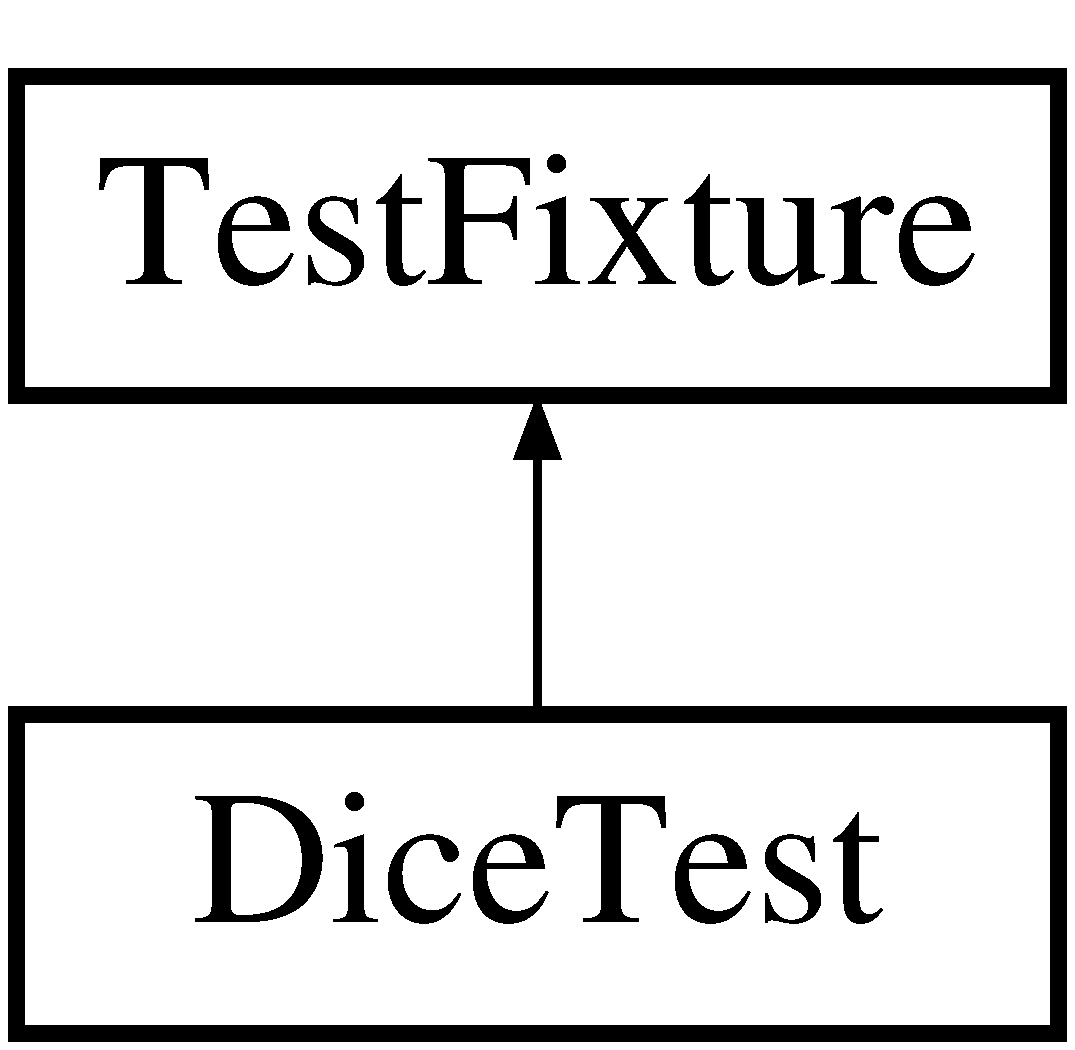
\includegraphics[height=2.000000cm]{class_dice_test}
\end{center}
\end{figure}
\subsection*{Protected Member Functions}
\begin{DoxyCompactItemize}
\item 
void \hyperlink{class_dice_test_a3e9f2421e914d4f18de2327828345860}{test\+Dice\+Roll\+Input\+Validity} ()
\item 
void \hyperlink{class_dice_test_a365b7b1d1ffe9faac8f306de9944d173}{test\+Dice\+Rolling\+Bounds} ()
\item 
void \hyperlink{class_dice_test_ac46b7044f229250c84b8dafaf432c80d}{test\+Invalid\+Dice\+Types} ()
\item 
void \hyperlink{class_dice_test_a849ab553a12a5a5d4deec59ddd1edf30}{test\+Multiple\+Dice} ()
\end{DoxyCompactItemize}
\subsection*{Private Member Functions}
\begin{DoxyCompactItemize}
\item 
\hypertarget{class_dice_test_ae60af42068499ec4e3dac71d8a7d31d5}{}\label{class_dice_test_ae60af42068499ec4e3dac71d8a7d31d5} 
{\bfseries C\+P\+P\+U\+N\+I\+T\+\_\+\+T\+E\+S\+T\+\_\+\+S\+U\+I\+TE} (\hyperlink{class_dice_test}{Dice\+Test})
\item 
\hypertarget{class_dice_test_ae60a88cf9ee33179fc1d7ba0d0ac27c9}{}\label{class_dice_test_ae60a88cf9ee33179fc1d7ba0d0ac27c9} 
{\bfseries C\+P\+P\+U\+N\+I\+T\+\_\+\+T\+E\+ST} (\hyperlink{class_dice_test_a3e9f2421e914d4f18de2327828345860}{test\+Dice\+Roll\+Input\+Validity})
\item 
\hypertarget{class_dice_test_a2114378e2f9228c529f19055c2b07d2b}{}\label{class_dice_test_a2114378e2f9228c529f19055c2b07d2b} 
{\bfseries C\+P\+P\+U\+N\+I\+T\+\_\+\+T\+E\+ST} (\hyperlink{class_dice_test_a365b7b1d1ffe9faac8f306de9944d173}{test\+Dice\+Rolling\+Bounds})
\item 
\hypertarget{class_dice_test_af30057a8554704368f119ab1a26c6e8a}{}\label{class_dice_test_af30057a8554704368f119ab1a26c6e8a} 
{\bfseries C\+P\+P\+U\+N\+I\+T\+\_\+\+T\+E\+ST} (\hyperlink{class_dice_test_ac46b7044f229250c84b8dafaf432c80d}{test\+Invalid\+Dice\+Types})
\item 
\hypertarget{class_dice_test_a7de775b83af7ea891c87c1203119c262}{}\label{class_dice_test_a7de775b83af7ea891c87c1203119c262} 
{\bfseries C\+P\+P\+U\+N\+I\+T\+\_\+\+T\+E\+ST} (\hyperlink{class_dice_test_a849ab553a12a5a5d4deec59ddd1edf30}{test\+Multiple\+Dice})
\item 
\hypertarget{class_dice_test_a8200325837de38fdee61cdec137b64a4}{}\label{class_dice_test_a8200325837de38fdee61cdec137b64a4} 
{\bfseries C\+P\+P\+U\+N\+I\+T\+\_\+\+T\+E\+S\+T\+\_\+\+S\+U\+I\+T\+E\+\_\+\+E\+ND} ()
\end{DoxyCompactItemize}


\subsection{Detailed Description}
Test Class for the \hyperlink{class_dice}{Dice} class. 

Definition at line 20 of file Dice\+Test.\+cpp.



\subsection{Member Function Documentation}
\hypertarget{class_dice_test_a365b7b1d1ffe9faac8f306de9944d173}{}\label{class_dice_test_a365b7b1d1ffe9faac8f306de9944d173} 
\index{Dice\+Test@{Dice\+Test}!test\+Dice\+Rolling\+Bounds@{test\+Dice\+Rolling\+Bounds}}
\index{test\+Dice\+Rolling\+Bounds@{test\+Dice\+Rolling\+Bounds}!Dice\+Test@{Dice\+Test}}
\subsubsection{\texorpdfstring{test\+Dice\+Rolling\+Bounds()}{testDiceRollingBounds()}}
{\footnotesize\ttfamily void Dice\+Test\+::test\+Dice\+Rolling\+Bounds (\begin{DoxyParamCaption}{ }\end{DoxyParamCaption})\hspace{0.3cm}{\ttfamily [protected]}}

test method for roll function of the \hyperlink{class_dice}{Dice} class Test Case\+: the upperbound of all values returned from roll function 

Definition at line 64 of file Dice\+Test.\+cpp.


\begin{DoxyCode}
65 \{
66     \textcolor{keywordtype}{int} result = 0;
67     \textcolor{keywordflow}{for} (\textcolor{keywordtype}{int} j = 1; j <= 1000; j++) \{
68         result= \hyperlink{class_dice_a4923bdf22040579e6e071e1e987916c2}{Dice::roll}(\textcolor{stringliteral}{"1d4"});
69         CPPUNIT\_ASSERT(result >= 1);
70         CPPUNIT\_ASSERT(result <= 4);
71     \}
72     \textcolor{keywordflow}{for} (\textcolor{keywordtype}{int} j = 1; j <= 1000; j++) \{
73         result = \hyperlink{class_dice_a4923bdf22040579e6e071e1e987916c2}{Dice::roll}(\textcolor{stringliteral}{"1d6"});
74         CPPUNIT\_ASSERT(result >= 1);
75         CPPUNIT\_ASSERT(result <= 6);
76     \}
77     \textcolor{keywordflow}{for} (\textcolor{keywordtype}{int} j = 1; j <= 1000; j++) \{
78         \textcolor{keywordtype}{int} numbers = \hyperlink{class_dice_a4923bdf22040579e6e071e1e987916c2}{Dice::roll}(\textcolor{stringliteral}{"1d8"});
79         CPPUNIT\_ASSERT(result >= 1);
80         CPPUNIT\_ASSERT(result <= 8);
81     \}
82     \textcolor{keywordflow}{for} (\textcolor{keywordtype}{int} j = 1; j <= 1000; j++) \{
83         \textcolor{keywordtype}{int} numbers = \hyperlink{class_dice_a4923bdf22040579e6e071e1e987916c2}{Dice::roll}(\textcolor{stringliteral}{"1d10"});
84         CPPUNIT\_ASSERT(result >= 1);
85         CPPUNIT\_ASSERT(result <= 10);
86     \}
87     \textcolor{keywordflow}{for} (\textcolor{keywordtype}{int} j = 1; j <= 1000; j++) \{
88         \textcolor{keywordtype}{int} numbers = \hyperlink{class_dice_a4923bdf22040579e6e071e1e987916c2}{Dice::roll}(\textcolor{stringliteral}{"1d12"});
89         CPPUNIT\_ASSERT(result >= 1);
90         CPPUNIT\_ASSERT(result <= 12);
91     \}
92     \textcolor{keywordflow}{for} (\textcolor{keywordtype}{int} j = 1; j <= 1000; j++) \{
93         \textcolor{keywordtype}{int} numbers = \hyperlink{class_dice_a4923bdf22040579e6e071e1e987916c2}{Dice::roll}(\textcolor{stringliteral}{"1d20"});
94         CPPUNIT\_ASSERT(result >= 1);
95         CPPUNIT\_ASSERT(result <= 20);
96     \}
97     \textcolor{keywordflow}{for} (\textcolor{keywordtype}{int} j = 1; j <= 1000; j++) \{
98         \textcolor{keywordtype}{int} numbers = \hyperlink{class_dice_a4923bdf22040579e6e071e1e987916c2}{Dice::roll}(\textcolor{stringliteral}{"1d100"});
99         CPPUNIT\_ASSERT(result >= 1);
100         CPPUNIT\_ASSERT(result <= 100);
101     \}
102 \}
\end{DoxyCode}
\hypertarget{class_dice_test_a3e9f2421e914d4f18de2327828345860}{}\label{class_dice_test_a3e9f2421e914d4f18de2327828345860} 
\index{Dice\+Test@{Dice\+Test}!test\+Dice\+Roll\+Input\+Validity@{test\+Dice\+Roll\+Input\+Validity}}
\index{test\+Dice\+Roll\+Input\+Validity@{test\+Dice\+Roll\+Input\+Validity}!Dice\+Test@{Dice\+Test}}
\subsubsection{\texorpdfstring{test\+Dice\+Roll\+Input\+Validity()}{testDiceRollInputValidity()}}
{\footnotesize\ttfamily void Dice\+Test\+::test\+Dice\+Roll\+Input\+Validity (\begin{DoxyParamCaption}{ }\end{DoxyParamCaption})\hspace{0.3cm}{\ttfamily [protected]}}

test method for roll function of the \hyperlink{class_dice}{Dice} class Test Case\+: the the validity of input string 

Definition at line 40 of file Dice\+Test.\+cpp.


\begin{DoxyCode}
41 \{
42     \textcolor{keywordtype}{int} result = 0;
43     
44     \textcolor{comment}{// test that if the string is valid, the result is calculated}
45     result = \hyperlink{class_dice_a4923bdf22040579e6e071e1e987916c2}{Dice::roll}(\textcolor{stringliteral}{"4d20"});
46     CPPUNIT\_ASSERT(result > 0);
47     result = \hyperlink{class_dice_a4923bdf22040579e6e071e1e987916c2}{Dice::roll}(\textcolor{stringliteral}{"3d10+1"});
48     CPPUNIT\_ASSERT(result > 0);
49 
50     \textcolor{comment}{//test that is the string is invalid, roll() returns -1}
51     result = \hyperlink{class_dice_a4923bdf22040579e6e071e1e987916c2}{Dice::roll}(\textcolor{stringliteral}{"4d"});
52     CPPUNIT\_ASSERT(result == -1);
53     result = \hyperlink{class_dice_a4923bdf22040579e6e071e1e987916c2}{Dice::roll}(\textcolor{stringliteral}{"d20"});
54     CPPUNIT\_ASSERT(result == -1);
55     result = \hyperlink{class_dice_a4923bdf22040579e6e071e1e987916c2}{Dice::roll}(\textcolor{stringliteral}{"420"});
56     CPPUNIT\_ASSERT(result == -1);
57     result = \hyperlink{class_dice_a4923bdf22040579e6e071e1e987916c2}{Dice::roll}(\textcolor{stringliteral}{"4d20+"});
58     CPPUNIT\_ASSERT(result == -1);
59 \}
\end{DoxyCode}
\hypertarget{class_dice_test_ac46b7044f229250c84b8dafaf432c80d}{}\label{class_dice_test_ac46b7044f229250c84b8dafaf432c80d} 
\index{Dice\+Test@{Dice\+Test}!test\+Invalid\+Dice\+Types@{test\+Invalid\+Dice\+Types}}
\index{test\+Invalid\+Dice\+Types@{test\+Invalid\+Dice\+Types}!Dice\+Test@{Dice\+Test}}
\subsubsection{\texorpdfstring{test\+Invalid\+Dice\+Types()}{testInvalidDiceTypes()}}
{\footnotesize\ttfamily void Dice\+Test\+::test\+Invalid\+Dice\+Types (\begin{DoxyParamCaption}{ }\end{DoxyParamCaption})\hspace{0.3cm}{\ttfamily [protected]}}

test method for roll function of the \hyperlink{class_dice}{Dice} class Test Case\+: rolling dice of invalid types (ie not d4, 6, 8, 10, 12, 20, 100) 

Definition at line 107 of file Dice\+Test.\+cpp.


\begin{DoxyCode}
108 \{
109     \textcolor{keywordtype}{int} result = 0;
110     result = \hyperlink{class_dice_a4923bdf22040579e6e071e1e987916c2}{Dice::roll}(\textcolor{stringliteral}{"2d9"});
111     CPPUNIT\_ASSERT(result == -1);
112     result = \hyperlink{class_dice_a4923bdf22040579e6e071e1e987916c2}{Dice::roll}(\textcolor{stringliteral}{"1d102"});
113     CPPUNIT\_ASSERT(result == -1);
114     result = \hyperlink{class_dice_a4923bdf22040579e6e071e1e987916c2}{Dice::roll}(\textcolor{stringliteral}{"4d17"});
115     CPPUNIT\_ASSERT(result == -1);
116     result = \hyperlink{class_dice_a4923bdf22040579e6e071e1e987916c2}{Dice::roll}(\textcolor{stringliteral}{"1d11"});
117     CPPUNIT\_ASSERT(result == -1);
118     result = \hyperlink{class_dice_a4923bdf22040579e6e071e1e987916c2}{Dice::roll}(\textcolor{stringliteral}{"1d62"});
119     CPPUNIT\_ASSERT(result == -1);
120     result = \hyperlink{class_dice_a4923bdf22040579e6e071e1e987916c2}{Dice::roll}(\textcolor{stringliteral}{"1d10000"});
121 \}
\end{DoxyCode}
\hypertarget{class_dice_test_a849ab553a12a5a5d4deec59ddd1edf30}{}\label{class_dice_test_a849ab553a12a5a5d4deec59ddd1edf30} 
\index{Dice\+Test@{Dice\+Test}!test\+Multiple\+Dice@{test\+Multiple\+Dice}}
\index{test\+Multiple\+Dice@{test\+Multiple\+Dice}!Dice\+Test@{Dice\+Test}}
\subsubsection{\texorpdfstring{test\+Multiple\+Dice()}{testMultipleDice()}}
{\footnotesize\ttfamily void Dice\+Test\+::test\+Multiple\+Dice (\begin{DoxyParamCaption}{ }\end{DoxyParamCaption})\hspace{0.3cm}{\ttfamily [protected]}}

test method for roll function of the \hyperlink{class_dice}{Dice} class Test Case\+: rolling multiple dice in one function call 

Definition at line 125 of file Dice\+Test.\+cpp.


\begin{DoxyCode}
126 \{
127     \textcolor{keywordflow}{for} (\textcolor{keywordtype}{int} j = 1; j <= 500; j++) \{
128         \textcolor{keywordtype}{int} result = \hyperlink{class_dice_a4923bdf22040579e6e071e1e987916c2}{Dice::roll}(\textcolor{stringliteral}{"2d6"});
129         CPPUNIT\_ASSERT(result >= 2);
130         CPPUNIT\_ASSERT(result <= 12);
131     \}
132 
133     \textcolor{keywordflow}{for} (\textcolor{keywordtype}{int} j = 1; j <= 500; j++) \{
134         \textcolor{keywordtype}{int} result = \hyperlink{class_dice_a4923bdf22040579e6e071e1e987916c2}{Dice::roll}(\textcolor{stringliteral}{"3d8"});
135         CPPUNIT\_ASSERT(result >= 3);
136         CPPUNIT\_ASSERT(result <= 24);
137     \}
138 
139     \textcolor{keywordflow}{for} (\textcolor{keywordtype}{int} j = 1; j <= 500; j++) \{
140         \textcolor{keywordtype}{int} result = \hyperlink{class_dice_a4923bdf22040579e6e071e1e987916c2}{Dice::roll}(\textcolor{stringliteral}{"4d10"});
141         CPPUNIT\_ASSERT(result >= 4);
142         CPPUNIT\_ASSERT(result <= 40);
143     \}
144 
145     \textcolor{keywordflow}{for} (\textcolor{keywordtype}{int} j = 1; j <= 500; j++) \{
146         \textcolor{keywordtype}{int} result = \hyperlink{class_dice_a4923bdf22040579e6e071e1e987916c2}{Dice::roll}(\textcolor{stringliteral}{"5d12"});
147         CPPUNIT\_ASSERT(result >= 5);
148         CPPUNIT\_ASSERT(result <= 60);
149     \}
150 
151     \textcolor{keywordflow}{for} (\textcolor{keywordtype}{int} j = 1; j <= 500; j++) \{
152         \textcolor{keywordtype}{int} result = \hyperlink{class_dice_a4923bdf22040579e6e071e1e987916c2}{Dice::roll}(\textcolor{stringliteral}{"6d20"});
153         CPPUNIT\_ASSERT(result >= 6);
154         CPPUNIT\_ASSERT(result <= 120);
155     \}
156 
157     \textcolor{keywordflow}{for} (\textcolor{keywordtype}{int} j = 1; j <= 500; j++) \{
158         \textcolor{keywordtype}{int} result = \hyperlink{class_dice_a4923bdf22040579e6e071e1e987916c2}{Dice::roll}(\textcolor{stringliteral}{"7d100"});
159         CPPUNIT\_ASSERT(result >= 7);
160         CPPUNIT\_ASSERT(result <= 700);
161     \}
162 \}
\end{DoxyCode}


The documentation for this class was generated from the following file\+:\begin{DoxyCompactItemize}
\item 
\hyperlink{_dice_test_8cpp}{Dice\+Test.\+cpp}\end{DoxyCompactItemize}

\chapter{File Documentation}
\hypertarget{dice_8cpp}{}\section{dice.\+cpp File Reference}
\label{dice_8cpp}\index{dice.\+cpp@{dice.\+cpp}}


\hyperlink{class_dice}{Dice} class implementation.  


{\ttfamily \#include \char`\"{}Dice.\+h\char`\"{}}\newline


\subsection{Detailed Description}
\hyperlink{class_dice}{Dice} class implementation. 


\hypertarget{dice_8h}{}\section{dice.\+h File Reference}
\label{dice_8h}\index{dice.\+h@{dice.\+h}}


Header file for the \hyperlink{class_dice}{Dice} class.  


{\ttfamily \#include $<$regex$>$}\newline
{\ttfamily \#include $<$iostream$>$}\newline
{\ttfamily \#include $<$random$>$}\newline
\subsection*{Classes}
\begin{DoxyCompactItemize}
\item 
class \hyperlink{class_dice}{Dice}
\begin{DoxyCompactList}\small\item\em \hyperlink{class_dice}{Dice} class. \end{DoxyCompactList}\end{DoxyCompactItemize}


\subsection{Detailed Description}
Header file for the \hyperlink{class_dice}{Dice} class. 


\hypertarget{_dice_test_8cpp}{}\section{Dice\+Test.\+cpp File Reference}
\label{_dice_test_8cpp}\index{Dice\+Test.\+cpp@{Dice\+Test.\+cpp}}


Implementation file for the \hyperlink{class_dice_test}{Dice\+Test} class.  


{\ttfamily \#include $<$cppunit/\+Test\+Case.\+h$>$}\newline
{\ttfamily \#include $<$cppunit/\+Test\+Fixture.\+h$>$}\newline
{\ttfamily \#include $<$cppunit/ui/text/\+Text\+Test\+Runner.\+h$>$}\newline
{\ttfamily \#include $<$cppunit/extensions/\+Helper\+Macros.\+h$>$}\newline
{\ttfamily \#include $<$cppunit/extensions/\+Test\+Factory\+Registry.\+h$>$}\newline
{\ttfamily \#include $<$cppunit/\+Test\+Result.\+h$>$}\newline
{\ttfamily \#include $<$cppunit/\+Test\+Result\+Collector.\+h$>$}\newline
{\ttfamily \#include $<$cppunit/\+Test\+Runner.\+h$>$}\newline
{\ttfamily \#include $<$cppunit/\+Brief\+Test\+Progress\+Listener.\+h$>$}\newline
{\ttfamily \#include $<$cppunit/\+Compiler\+Outputter.\+h$>$}\newline
{\ttfamily \#include $<$cppunit/\+Xml\+Outputter.\+h$>$}\newline
{\ttfamily \#include \char`\"{}Dice.\+h\char`\"{}}\newline
\subsection*{Classes}
\begin{DoxyCompactItemize}
\item 
class \hyperlink{class_dice_test}{Dice\+Test}
\begin{DoxyCompactList}\small\item\em Test Class for the \hyperlink{class_dice}{Dice} class. \end{DoxyCompactList}\end{DoxyCompactItemize}
\subsection*{Functions}
\begin{DoxyCompactItemize}
\item 
\hypertarget{_dice_test_8cpp_a3ac77e5cf1043b4a814c2bef908a9cdd}{}\label{_dice_test_8cpp_a3ac77e5cf1043b4a814c2bef908a9cdd} 
\hyperlink{_dice_test_8cpp_a3ac77e5cf1043b4a814c2bef908a9cdd}{C\+P\+P\+U\+N\+I\+T\+\_\+\+T\+E\+S\+T\+\_\+\+S\+U\+I\+T\+E\+\_\+\+R\+E\+G\+I\+S\+T\+R\+A\+T\+I\+ON} (\hyperlink{class_dice_test}{Dice\+Test})
\begin{DoxyCompactList}\small\item\em cppunit test cases registration \end{DoxyCompactList}\end{DoxyCompactItemize}


\subsection{Detailed Description}
Implementation file for the \hyperlink{class_dice_test}{Dice\+Test} class. 


\hypertarget{_run_app_8cpp}{}\section{Run\+App.\+cpp File Reference}
\label{_run_app_8cpp}\index{Run\+App.\+cpp@{Run\+App.\+cpp}}


Driver file to create and execute the test suite.  


{\ttfamily \#include $<$cppunit/\+Compiler\+Outputter.\+h$>$}\\*
{\ttfamily \#include $<$cppunit/extensions/\+Test\+Factory\+Registry.\+h$>$}\\*
{\ttfamily \#include $<$cppunit/ui/text/\+Test\+Runner.\+h$>$}\\*
\subsection*{Functions}
\begin{DoxyCompactItemize}
\item 
int \hyperlink{_run_app_8cpp_a0ddf1224851353fc92bfbff6f499fa97}{main} (int argc, char $\ast$argv\mbox{[}$\,$\mbox{]})
\end{DoxyCompactItemize}


\subsection{Detailed Description}
Driver file to create and execute the test suite. 

Brief instruction on how to set Cpp\+Unit\+: from\+: http \+://www.comp.\+nus.\+edu.\+sg/$\sim$cs3215/tools/cppunit\+All.html

First, to install cpp\+Unit \+:


\begin{DoxyEnumerate}
\item Unpack the Cpp\+Unit archive (\href{https://sourceforge.net/projects/cppunit/files/cppunit/1.12.1/}{\tt https\+://sourceforge.\+net/projects/cppunit/files/cppunit/1.\+12.\+1/}) to a directory of your choice, in this example I assume it is D\+:.
\item Go to D\+:/cppunit-\/1.12.\+1/src and open the Cpp\+Unit\+Libraries.\+dsw in Visual Studio.
\item Select the cppunit project in the Solution Explorer and go to 'Project $>$ Properties $>$ Configuration Properties $>$ Librarian $>$ General. Put \char`\"{}\+Debug\textbackslash{}cppunit.\+lib\char`\"{} in the �\+Output File� textbox.
\item Right-\/click on the cppunit project in the Solution Explorer pane and choose Build.
\item After successful compilation, D\+:/cppunit-\/1.12.\+1/lib/cppunit.lib is produced which you then need to setup the Visual Studio Linker with (see below). 
\end{DoxyEnumerate}

\subsection{Function Documentation}
\hypertarget{_run_app_8cpp_a0ddf1224851353fc92bfbff6f499fa97}{}\index{Run\+App.\+cpp@{Run\+App.\+cpp}!main@{main}}
\index{main@{main}!Run\+App.\+cpp@{Run\+App.\+cpp}}
\subsubsection[{main}]{\setlength{\rightskip}{0pt plus 5cm}int main (
\begin{DoxyParamCaption}
\item[{int}]{argc, }
\item[{char $\ast$}]{argv\mbox{[}$\,$\mbox{]}}
\end{DoxyParamCaption}
)}\label{_run_app_8cpp_a0ddf1224851353fc92bfbff6f499fa97}
To setup a project from scratch for Compilation / Linking\+:


\begin{DoxyEnumerate}
\item Activate 'Project $>$ Properties $>$ C/\+C++ $>$ Code Generation $>$ Runtime Library $>$ Multi -\/ threaded Debug D\+L\+L'
\item Go to 'Project $>$ Properties $>$ C/\+C++ $>$ General'. Put \char`\"{}\+D\+:\textbackslash{}cppunit-\/1.\+12.\+1\textbackslash{}include\char`\"{} in the 'Additional Include Directories' text box.
\item Go to 'Project $>$ Properties $>$ Linker $>$ Input'. Put \char`\"{}\+D\+:\textbackslash{}cppunit-\/1.\+12.\+1\textbackslash{}lib\textbackslash{}cppunit.\+lib\char`\"{} in the 'Additional Dependences' text box.
\item Go to 'Project $>$ Properties $>$ Build Events $>$ Post-\/\+Build Event'. Put '\char`\"{}\$(\+Target\+Path)\char`\"{}' in the 'Command Line' textbox.\+Put 'Unit Tests...' in the 'Description' textbox. \hyperlink{_run_app_8cpp_a0ddf1224851353fc92bfbff6f499fa97}{main()} function. Entry point of the program It does the following\+:
\end{DoxyEnumerate}

Create a test suite object from the registry as populated by the code in the Test Classes
\begin{DoxyEnumerate}
\item Create a test runner that will execute all the tests in the registry
\item (optionally) sets an outputter that will output the results
\item Run the test cases. 
\end{DoxyEnumerate}
%--- End generated contents ---

% Index
\backmatter
\newpage
\phantomsection
\clearemptydoublepage
\addcontentsline{toc}{chapter}{Index}
\printindex

\end{document}
